\documentclass[11pt, a4paper]{article}
\usepackage{amsmath}
\usepackage{amssymb}
\usepackage{amsthm}
\usepackage{epsfig}
\usepackage[margin=1in]{geometry}
\usepackage{enumitem}
% \usepackage{enumerate}
\usepackage{graphicx}

%%%%%%%%%% Package for Highlight         %%%%%%%
\usepackage[usenames, dvipsnames]{xcolor}


%%%%%%%%% Reference Style Here %%%%%%%%%%%%%%%%%%%%%%%%%

\usepackage[utf8]{inputenc}
\usepackage{csquotes}
\usepackage[english]{babel}
\usepackage[backend=biber,style=numeric,sorting=none]{biblatex}
\addbibresource{Reference.bib}

%%%%%%%%%%%%%%%%%%%%%%%%%%%%%%%%%%%%%%%%%%%%%%%%
\usepackage{tikz}
\usetikzlibrary{automata, positioning}
\usepackage{caption}
\usepackage{mathtools}
\usepackage{algorithm}
\usepackage{algorithmic}
\usepackage{todonotes}
\usepackage{times}
\usepackage{pdfpages}
\usepackage{mathtools}
%\usepackage[]{algorithm2e}

\usepackage{lipsum} % paragraph spacing
\usepackage{titlesec} % paragraph spacing
\usepackage{comment}
%%%%%%%%%%% CHINESE TYPING  %%%%%%%%%%%%
\usepackage{CJK} 
% How to use: 
% \begin{CJK}{UTF8}{} 
% \end{CJK}
%%%%%%%%%%%%%%%%%%%%%%%%%%%%%%%%%%%%%%%%%%%

%%%%%%%%%%%%%%%%%%%%%%%%%%
% 3 Columns & landscape	 %
%%%%%%%%%%%%%%%%%%%%%%%%%%
%\usepackage{multicol}
%\usepackage{pdflscape}

% For writing code:
\usepackage{fancyvrb}
\DefineVerbatimEnvironment{code}{Verbatim}{fontsize=\small}
\def\showvrb#1{%
	\texttt{\detokenize{#1}}%
}

\linespread{1.0}
\setlength{\parindent}{0pt} % Sets the indent length to 0
\setlength{\parskip}{0pt plus 1pt minus 1pt} % paragraph vertical distance

\everymath{\displaystyle} % displays inline math as displaymath

\hyphenpenalty=10000 % force no hyphenation



\begin{comment}
%%%%%%%%%%%%%%%%%%%%%%%%%%%%%%%%%
% ONLY RECOMMENDED FOR 3 COLUMN %
%%%%%%%%%%%%%%%%%%%%%%%%%%%%%%%%%%%%%%%%%%%%%%%%%%%%%%%%%%%%%%%%%%%%%

\setlist[itemize]{noitemsep, topsep=0pt, leftmargin=0.2in} % compacts lists with no item separation,indent from the left side = 0.2
\titlespacing\section{1pt}{5pt plus 4pt minus 2pt}{2pt plus 2pt minus 2pt}%paragraph spacing
\titlespacing\subsection{0pt}{5pt plus 4pt minus 2pt}{2pt plus 2pt minus 2pt}%paragraph spacing
\titlespacing\subsubsection{0pt}{5pt plus 4pt minus 2pt}{2pt plus 2pt minus 2pt}%paragraph spacing
\end{comment}


%%%%%%%%%%%%%%%% Normally use this! %%%%%%%%%%%%%%%%%%%%%%%%%%%%%%%%%%%%%%%%%%%%%%%%%%%%
%
\setlist[itemize]{noitemsep, topsep=3pt} % compacts lists with no item separation    %%%
%
%
%%%%%%%%%%%%%%%%%%%%%%%%%%%%%%%%%%%%%%%%%%%%%%%%%%%%%%%%%%%%%%%%%%%%%%%%%%%%%%%%%%%%%%%%


\title{Performance Gap}
\author{Ying He}

%%%%%%%%%%%%%%%%%%%%%%%%%%%%%%%
%   Commonly used theorems    %
%%%%%%%%%%%%%%%%%%%%%%%%%%%%%%%

% Use roman for text - numbering follows onwards
\theoremstyle{definition}
\newtheorem{defn}{Definition}[section]
\newtheorem{them}{Theorem}[section]
\newtheorem{lem}{Lemma}[them]
\newtheorem{prop}[them]{Proposition}
\newtheorem{corr}[them]{Corollary}
\newtheorem{corrr}{Corollary}[them] %for consistency issues
% examples follow different numbering
\newtheorem{eg}{Example}[section]
\newtheorem{egg}[them]{Example}
\newtheorem*{themf}{Theorem 5.0}
\newtheorem*{themm}{Theorem}
\newtheorem{question}{Question}

%%%%%%%%%%%%%
% Shortcuts %
%%%%%%%%%%%%%

\newcommand{\Q}{\mathbb{Q}}
\newcommand{\C}{\mathbb{C}}
\newcommand{\F}{\mathbb{F}}
\newcommand{\R}{\mathbb{R}}
\newcommand{\Z}{\mathbb{Z}}
\newcommand{\N}{\mathbb{N}}
\newcommand{\D}{\mathbb{D}}

\newcommand{\mcC}{\mathcal{C}}
\newcommand{\mcN}{\mathcal{N}}
\newcommand{\mcE}{\mathcal{E}}
\newcommand{\mcP}{\mathcal{P}}
\newcommand{\mcF}{\mathcal{F}}
\newcommand{\mcS}{\mathcal{S}}
\newcommand{\mcA}{\mathcal{A}}
\newcommand{\mcB}{\mathcal{B}}
\newcommand{\mcX}{\mathcal{X}}
\newcommand{\mcL}{\mathcal{L}}
\newcommand{\mcH}{\mathcal{H}}
\newcommand{\mcl}{\mathcal{l}}

\newcommand{\bfe}{\mathbf{e}}
\newcommand{\mbf}{\mathbf}

\newcommand{\ran}{\mbox{Ran}}

\newcommand{\al}{\alpha}
\newcommand{\s}{\sigma}
\newcommand{\ep}{\epsilon}
\newcommand{\dl}{\delta}
\newcommand{\sg}{\sigma}

\newcommand{\bs}{\backslash}
\newcommand{\n}{\\}
\newcommand{\ol}{\overline}
%\newcommand{\bb}{\textbf} %Bold front
%\newcommand{\ul}{\underline} %underline

\newcommand{\ltlU}{\textsf{ \bfseries UNTIL }}
\newcommand{\ltlF}{\textsf{\bfseries F }}
\newcommand{\ltlG}{\textsf{\bfseries G }}
\newcommand{\ltlX}{\textsf{\bfseries X }}
\newcommand{\ltlA}{\textsf{\bfseries A }}
\newcommand{\ltlE}{\textsf{\bfseries E }}

%%%%%%%%%%%%%%%%%%%%%%%%%
% Standard big brackets %
%%%%%%%%%%%%%%%%%%%%%%%%%

\newcommand{\floor}[1]{\left\lfloor{#1}\right\rfloor}
\newcommand{\ceil}[1]{\left\lceil{#1}\right\rceil}
\newcommand{\bbA}[1]{\left({#1}\right)}
\newcommand{\bbB}[1]{\left[{#1}\right]}
\newcommand{\bbC}[1]{\left\{{#1}\right\}}



%%%%%%%%%%%%%%%%%
%  MATRIX       %
%%%%%%%%%%%%%%%%%
\newcommand{\matxx}[9]{\begin{pmatrix} #1 & #2 & #3 \\ #4 & #5 & #6 \\ #7 & #8 & #9 \end{pmatrix}}
\newcommand{\matx}[4]{\begin{pmatrix} #1 & #2 \\ #3 & #4 \end{pmatrix}}
%example
%    $\matx{1}{2}{3}{4}{5}{6}{7}{8}{9}$

%%%%%%%%%%%%%%%%

%%%%%%%%%%%%%%%%%%%%%%%%%%%%%
% Highlight color
%%%%%%%%%%%%%%%%%%%%%%%%%%%

\newcommand{\hgy}{\colorbox{GreenYellow}} % Light Green
\newcommand{\hyg}{\colorbox{YellowGreen}} % another Light Green
\newcommand{\hlb}{\colorbox{SkyBlue}} % light blue
\newcommand{\hpink}{\colorbox{pink}} % Light pink
\newcommand{\hor}{\colorbox{orange}} % Orange
\newcommand{\hlor}{\colorbox{Apricot}} % Light Orange




%%%%%%%%%%%%%%%% SET Graphics Path %%%%%%%%%%%%%%
\graphicspath{{./Figure/}}




%%%%%%%%%%%%%%%%%%
% Start Document %
%%%%%%%%%%%%%%%%%%

\begin{document}
\begin{comment}
	\begin{landscape}
	\begin{multicols*}{3}
\end{comment}

\begin{comment}
\textbf{abcdefg}



%\tableofcontents


\hlor{abcd}

\[\matx{1}{2}{3}{4}\] al;dfjajfa

woyaozaizhedazi $\matx{1}{2}{3}{4}$



\[\alpha \cdot \beta \]
123456789/*
\end{comment}
\maketitle

\newpage
\tableofcontents

\section{Abstract}
This thesis aims to reduce the deviation between calculated and measured heating demands. A residential building and an office building are accurately modeled and calculated using EnergyPlus and SIA 180 standard. Both buildings are firstly calibrated based on historical annual heating demand and hourly indoor temperature, then several key building parameters are changed into different values. Based on the a large number of simulations, the result indicated that the most influential parameters in simulation are key area temperature heating set points, external wall solar absorptance, infiltration and lighting schedule. In order to reduce the performance gap, it is recommended to create an accurate building envelope and apply accurate outdoor environment. Therefore, an update to SIA standard weather data is also recommended.
\cite{FREI2017421}

\section{Introduction}
	\subsection{Background}
		Building simulation are widely used for different purposes such as to benchmark buildings or to evaluate energy demands and indoor thermal comforts. However, due to a number of factors, there are always deviations between calculated value and measurement value, which is also called \textbf{performance gap}. Previous studies which used standardized method \textbf{SIA 180/1} to calculate the heating demand of several buildings observed considerably large performance gap in uninsulated buildings.
	
	\subsection{Purpose and scope of this thesis}
		Therefore, the purpose of this thesis is to find out the main causes of the performance gap in uninsulated buildings, as well as the most influential factors in building simulation. In addition, this thesis also aim to investigate how the resulting energy demand variations affect the performance gap.

	\subsection{Description of this thesis}
		Two uninsulated buildings, one residential and one office buildings, are carefully modeled and analyzed using different approaches including SIA 180/1 calculation and EnergyPlus simulation. The buildings is firstly calibrated to match the historical measurement, then building parameters are modified and the most influential factors can be discovered.


	\subsection{Office Building Introduction}
		
		\begin{figure}[h!]
		\centering
		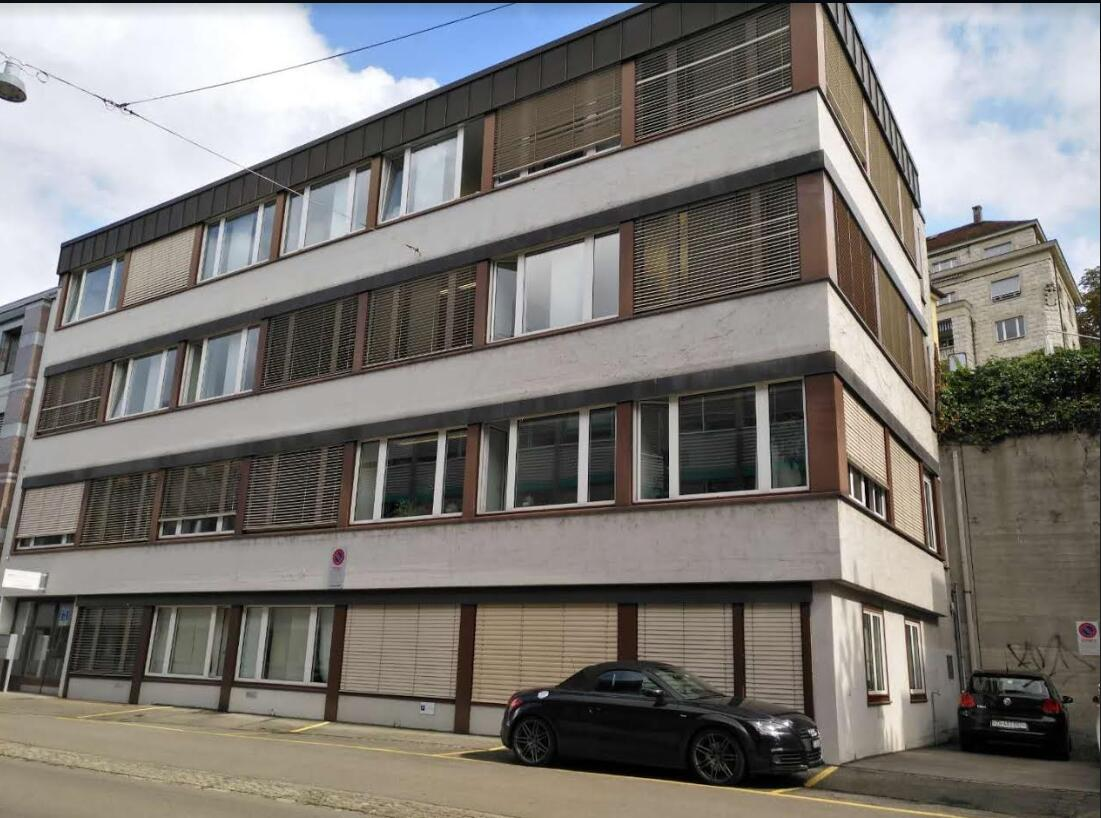
\includegraphics[scale=0.3]{Sumatra_photo.jpg}
		\caption{Sumatrastrasse 10 Office Building}
		\label{fig:Sumatra_photo}
		\end{figure}
		 
		
		According to the given information, the office building is constructed in 1951 and is located at Sumatrastrasse 10, 8006 Zurich, Switzerland. The building has 4 floors and a basement. The building  is facing west, and the window-to-wall ratio is 59\% on its west and south facade. The east facade of its ground floor and first floor is submerged into ground and there are heavy cover of plants on the upper floors with only a few necessary windows. There is also an underground floor used as warehouse and it's not included in any building model in this thesis.\\

		Figure \ref{fig:sumatra_og2} and \ref{fig:sumatra_og3} below are the floor plans of the building.
		The floor layout of ground floor, first floor and second floor are thought to be identical, and the third would have some small differences. For each floor, there is a toilet, a small office and 2 middle offices and a staircase. There is also a big office in each floor at the south side at ground floor, first floor and second floor. At the third floor, part of the big office and the corridor become a meeting room and a small pastry area as shown in the figures below. The detail building envelope material and modelling parameters are at Chapter \textbf{Methodology}.
		
		\begin{figure}[H]
		  \centering
		  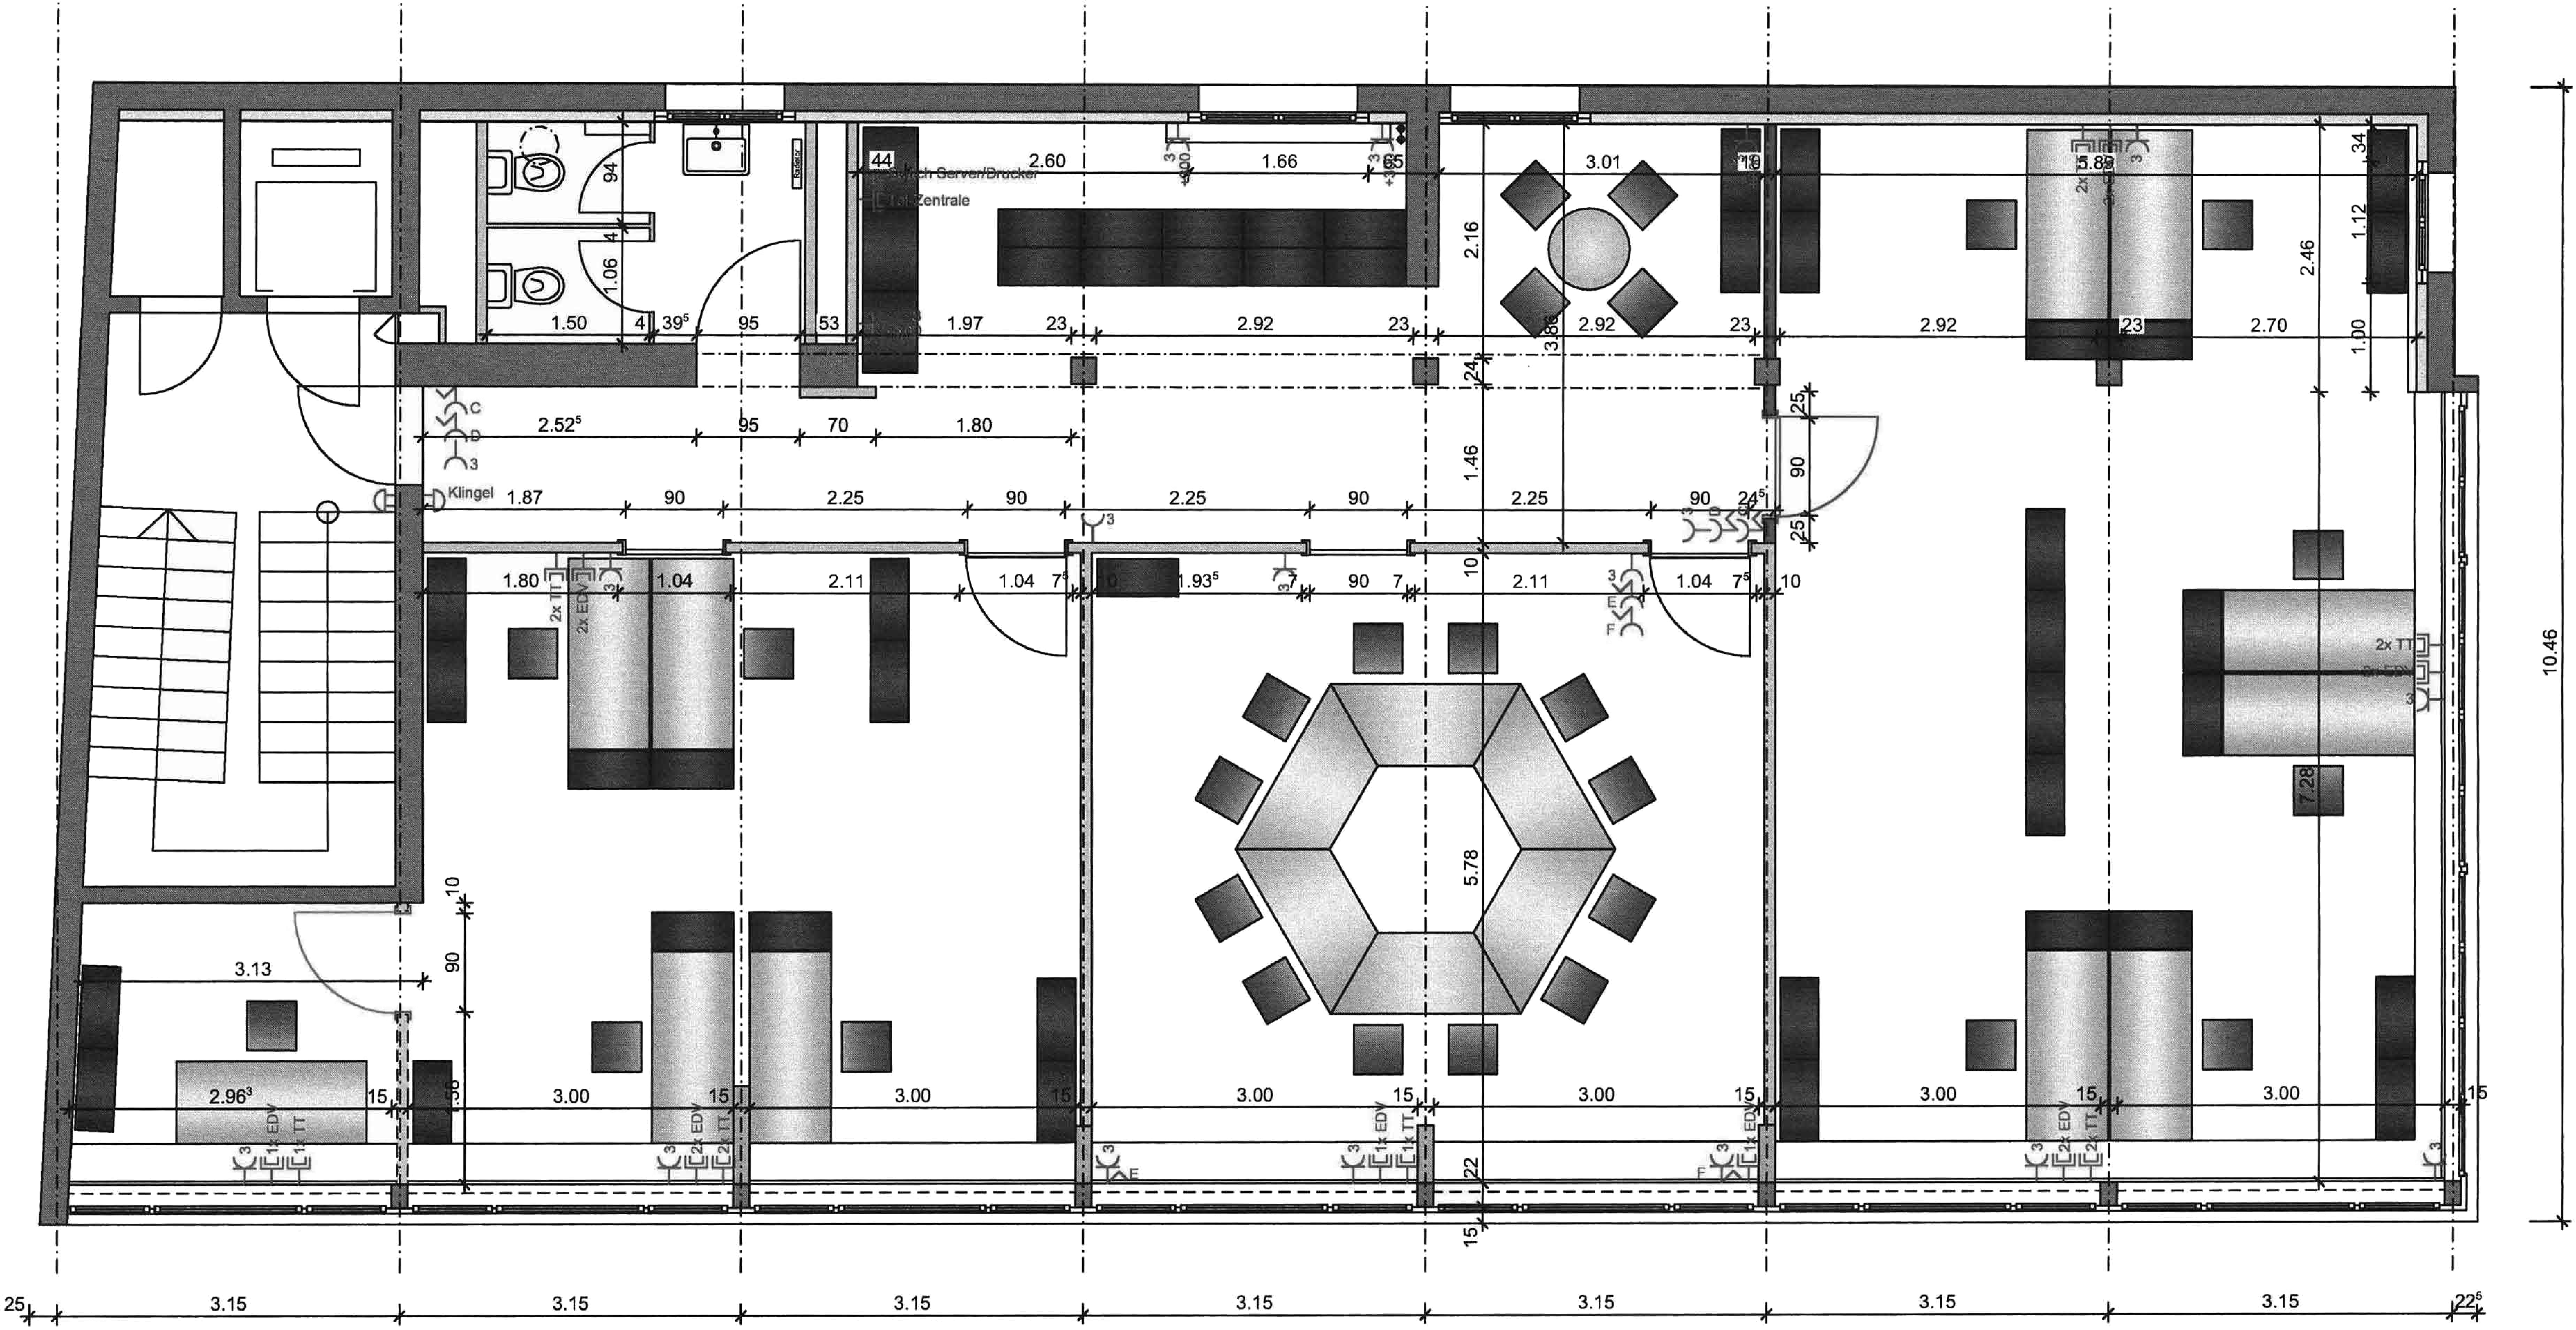
\includegraphics[scale=0.13]{Sumatra_OG2_Plan.pdf}
		  \caption{Floor plan of office building (Sumatra) ground floor to 2$^{nd}$ floor}
		  \label{fig:sumatra_og2}
		 \end{figure}

		\begin{figure}[H]
		  \centering
		  \includegraphics[scale=0.13]{Sumatra_OG3_Plan.pdf}
		  \caption{Floor plan of office building (Sumatra) 3$^{rd}$ floor}
		  \label{fig:sumatra_og3}
		\end{figure}
		
	\subsection{Residential Building Introduction}
		Figure \ref{fig:hongg_NE} and \ref{fig:hongg_SW} below show the photo of the residential building. The residential building is a part of a multi-family town house constructed in 1894. It is located at Honggerstrasse 23, 8037 Zurich, Switzerland. The building has 5 floors, the top floor is a loft and there is also an extra basement. There are 4 apartments in the building. The first apartment occupies the ground floor and the first floor, and the other 3 apartments each occupy one floor. Figure \ref{fig:hongg_eg_plan} and Figure \ref{fig:hongg_og1_plan} below are the floor plans of the residential building. The ground floor is connected with the first floor internally via a small staircase behide the kitchen. The black and red lines in Figure \ref{fig:hongg_eg_plan} show the ground floor layout and the yellow line indicates the layout of the upper floor. Similarily, Figure \ref{fig:hongg_og1_plan} shows the floor plans from first floor upward. The  red line indicates the layout of first floor and the yellow line shows the layout from second floor up. The detail building envelope material and modelling parameters are at Chapter \textbf{Methodology}.\\
		

		\begin{figure}[htbp]
		\centering
		\begin{minipage}[t]{0.48\textwidth}
		\centering
		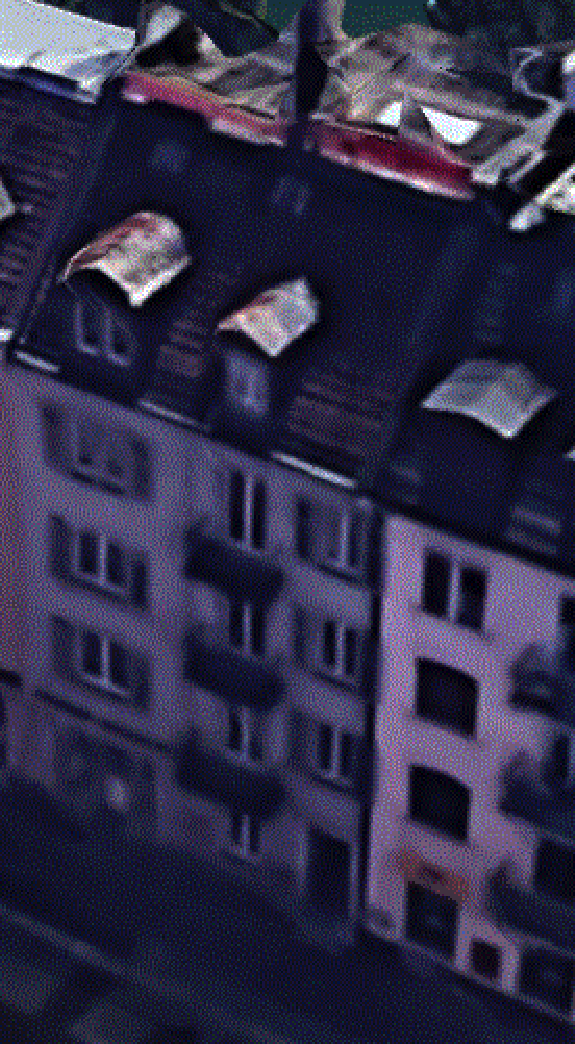
\includegraphics[width=5cm]{Hongg_photo1.pdf}
		\caption{Honggerstrasse 23, NE Side}
		\label{fig:hongg_NE}
		\end{minipage}
		\begin{minipage}[t]{0.48\textwidth}
		\centering
		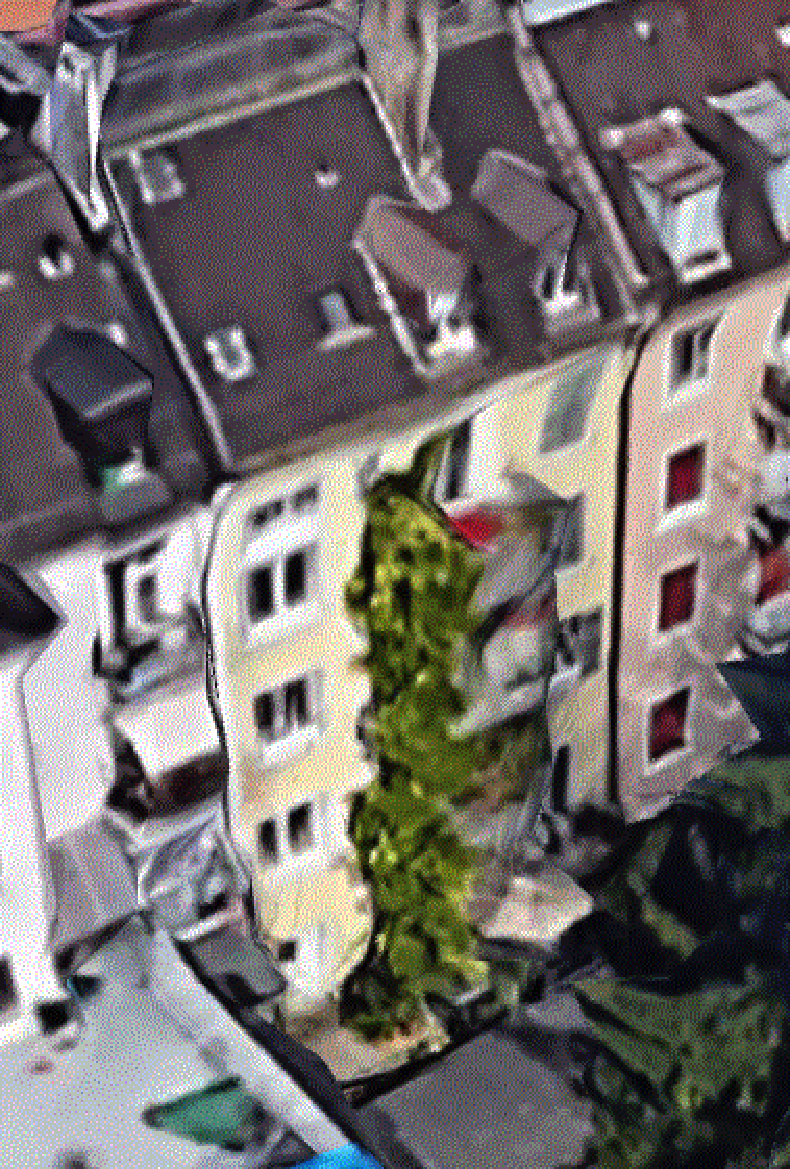
\includegraphics[width=6cm]{Hongg_photo0.pdf}
		\caption{Honggerstrasse 23, SW side}
		\label{fig:hongg_SW}
		\end{minipage}
		\end{figure}

		\begin{figure}[H]
		\centering
		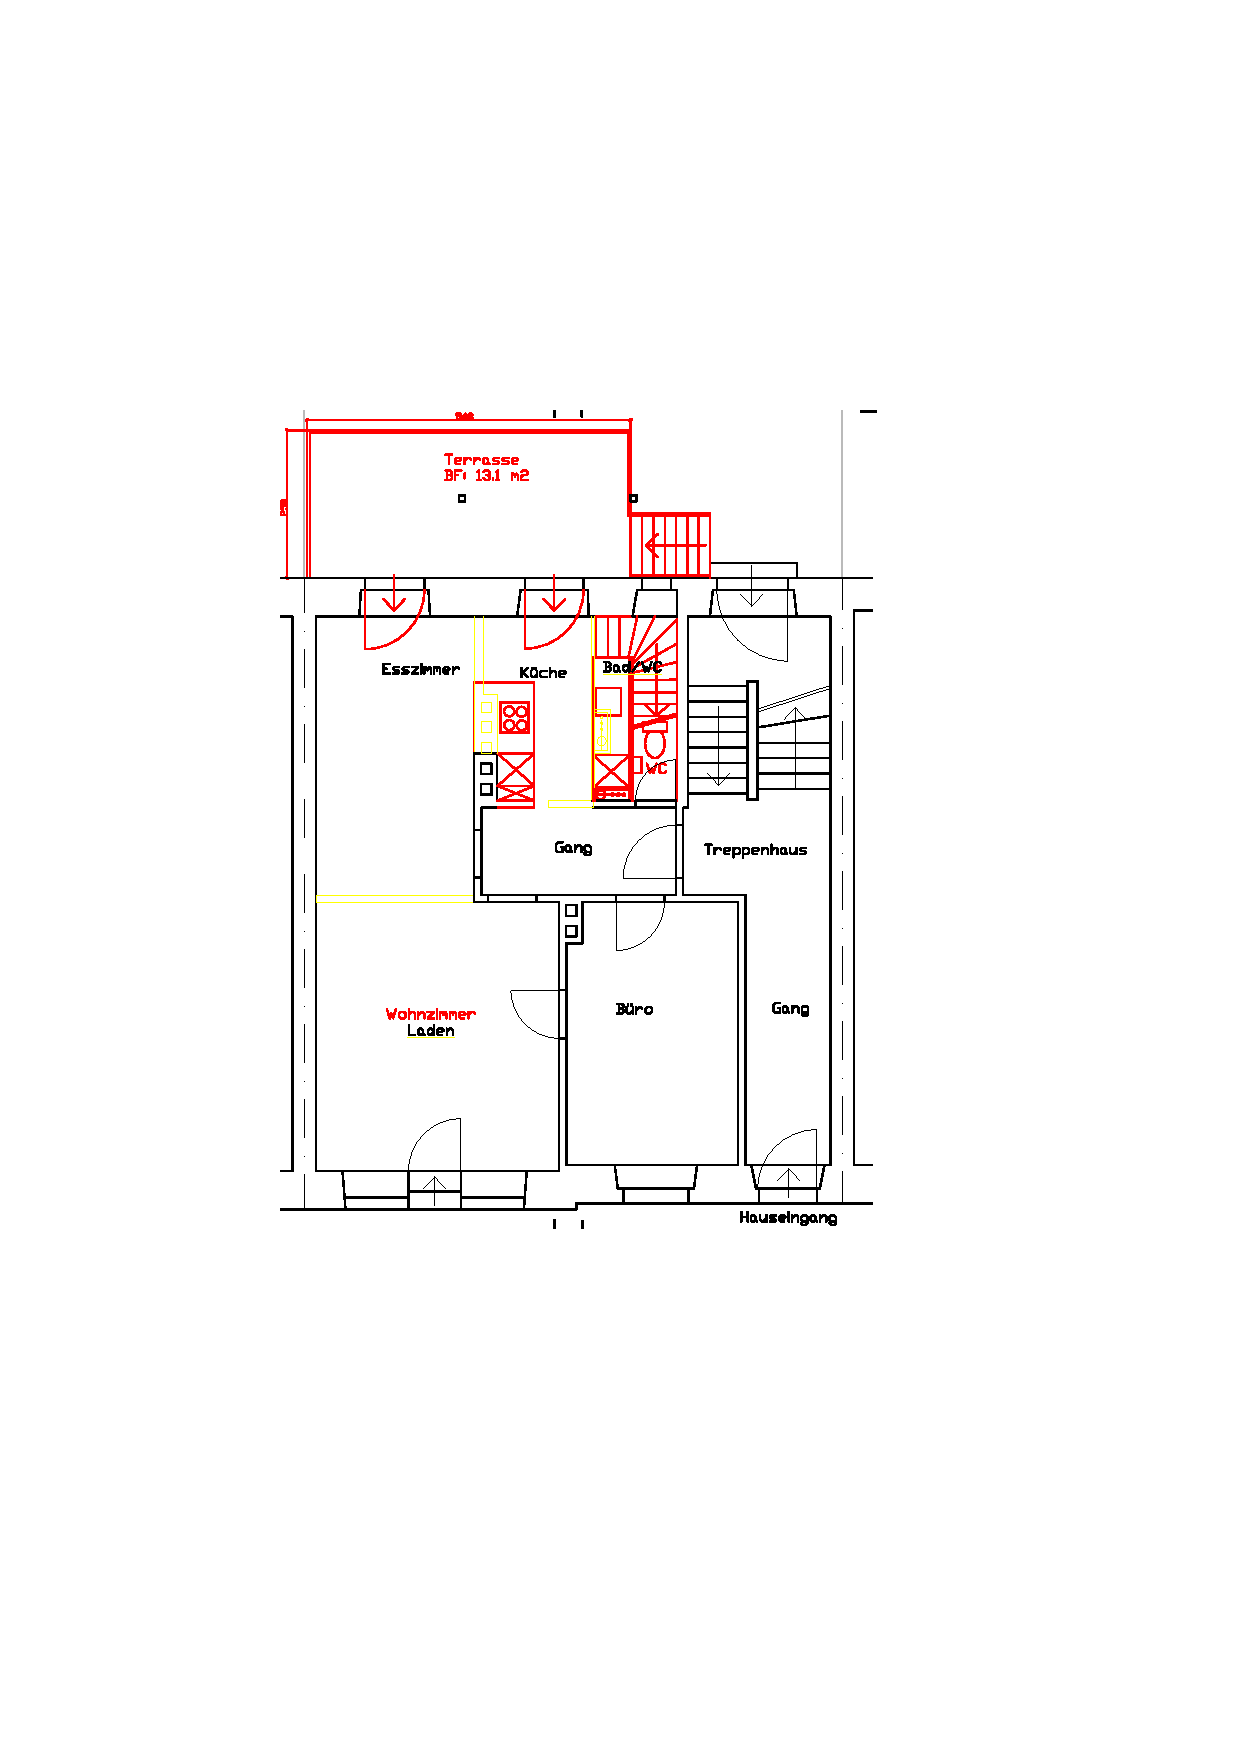
\includegraphics[scale=0.9]{Hongg_EG_Plan.pdf}
		\caption{Floor plan of residential building (Hongger) ground - 1$^{st}$ floor}
		\label{fig:hongg_eg_plan}
		\end{figure}
		
		\begin{figure}[H]
		\centering
		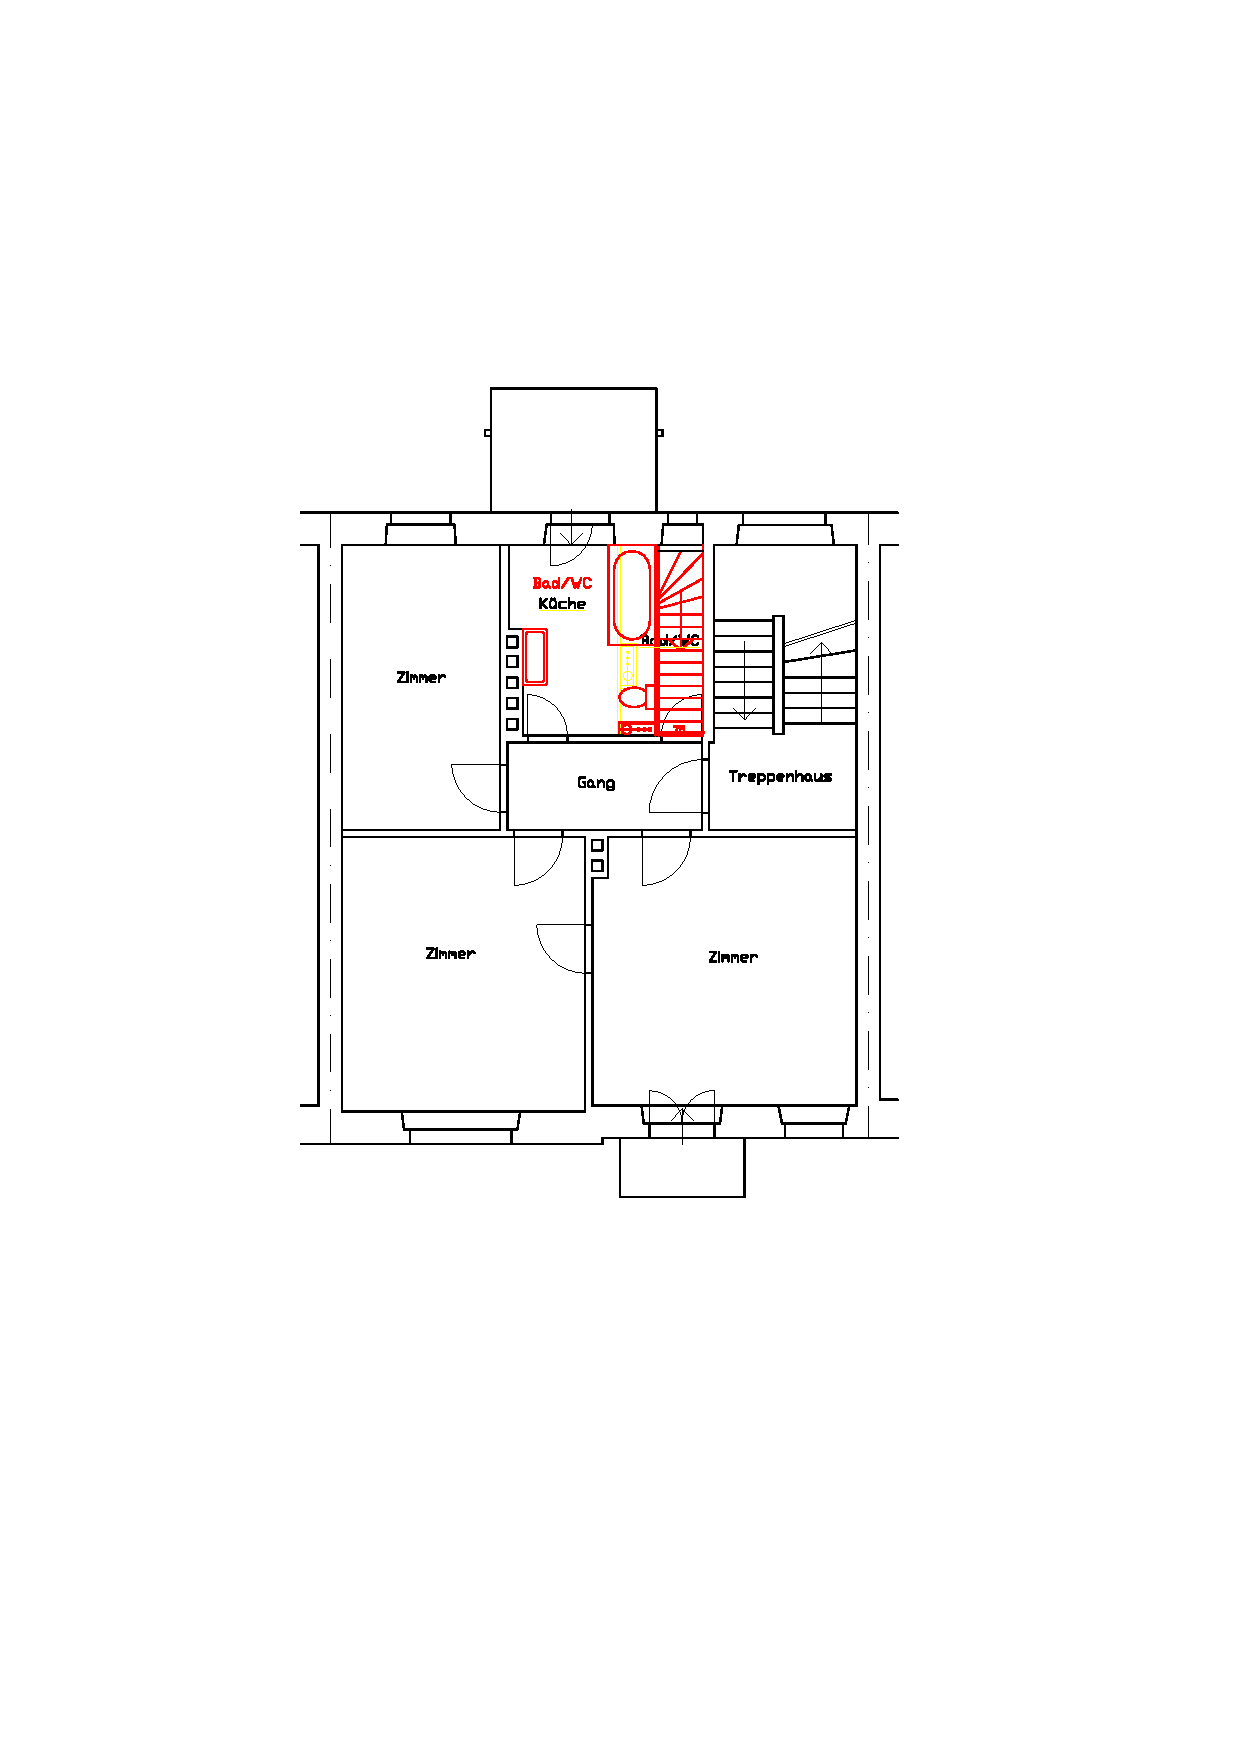
\includegraphics[scale=0.9]{Hongg_1OG_Plan.pdf}
		\caption{Floor plan of residential building (Hongger) 1$^{st} - 4^{th}$ floor}
		\label{fig:hongg_og1_plan}
		\end{figure}
		
\section{Literature Review}

	Over the past years, there are a large number of research about building energy performance gap (BEPG). Performance gap can cause problems in energy management system. However, the root cause of this gap is not clearly identified, and the gap can't be effectively managed and eliminated \cite{FREI2017421}.
	According to a recent review of these research , most of them would contain one or more of the following 5 elements: (1) building type, which can be classified as residential and non-residential, or even more specific types such as single-family house, multi-family house, office building, commercial building, hospital, prison, etc; (2) strategies for closing performance gap, which focus about design concept, technology and method, and "soft" measures; (3) building life cycle, which analyses the cause of performance gap in different stages of a building; (4) energy-related stakeholders, whose behavior would affect the performance gap; (5) the influence factors or building parameters that would cause or affect the performance gap \cite{FREI2017421}. Consider the objective of this thesis, the focus is on these following topics.
	
	\subsection{Root Causes of Performance Gap}
		Most causes of performance gap can be grouped into 3 categories base on the stages in the building life-cycle. They are design and simulation problems, misbehavior of contractors and misbehavior of building users \cite{userevaluations,NIU2016275}.\\
		
		\subsubsection{Design and simulation problem}
		Firstly, in most cases, building designers are account for the wrong doings in design and simulation processes. These include wrong assumptions and predictions about their design such as inaccurate building unheated area's temperature, wrong representation of user behavior, and wrong forecast of outdoor environment \cite{HOFFMANN201731,NIU2016275}. Also, it is difficult to predict the future environment such as climate, weather, and solar activities, which factors can lead to huge performance gaps \cite{DIAZ2017393,doi:10.1080/19401493.2012.718797}. For example, rainfall would greatly increase the heat convection coefficient of building facade surface, and therefore increase heat exchange rate through the building envelope \cite{DIAZ2017393}. In addition, the actual thermal performance of building materials subject from different factors and are usually perform worse than how they should in lab environments. Therefore, designers usually overestimate the actual performance of technology and apply inappropriate assumptions about user behaviors \cite{DEWILDE201440}. \\

		\subsubsection{Contractors}
		Secondly, contractors are mainly account for performance gaps caused by low quality constructions. Poor building quality and poor workmanship will usually reduce the thermal performance and therefore require more energy to maintain indoor comfort. Additionally, performance gap can be caused by contractors when they use improper construction techniques and when they are unable to discover hidden problems due to time and budget constraints \cite{DEWILDE201440}.In some cases, these problems would lead to huge building parameter deviations and therefore higher energy consumption than the design value \cite{FREI2017421,DEWILDE201440}. \\

		\subsubsection{User behaviors}
		Lastly, as the last and main stage of building's life-cycle, different behaviors of building users are also important sources of performance gap \cite{ZOU2018165}. These behaviors, either deliberate or unconscious, are usually not the optimum ways to operate a building. Building owners or occupants have specific behaviors due to their social and personal characteristics, attitude, experience, and thermal comfort standard \cite{userevaluations,LAWRENCE2016651}. For example, users may leave unnecessary appliance on without notice or open the windows when heatings or cooling system is operating \cite{FREI2017421}.\\

	\subsection{Strategies For Closing Performance Gap} 
		When the causes of performance gap are found out, strategies for closing the gap can also be developed. These strategies are grouped into 3 categories, which is, namely, design concept, technology and methods, and "soft" measures \cite{ZOU2018165}.\\

		\subsubsection{Design Concept}
			\textit{Passive design} is thought to be able to eliminate or decrease the impact of user behavior on energy consumption. Its philosophy is that if a building is designed in a way that no active equipment is needed, user behaviors would not influence the passive mechanism \cite{BLIGHT2013183,NORFORD1994121}. However, this approach has high construction quality requirements and can only have positive effects when both building designers and the occupants fully understand the building energy system. If building designers have inaccurate information about occupants, or building constructors don't have the capability to construct the building according to the specifications, or if the occupants do not fully understand the building system, passive design approach can only have adverse impacts \cite{ZOU2018165}.\\

			\textit{Active design}, on the other hand, use building automation system to improve occupants' thermal comfort and hopefully reduce the chance of wrong operations by occupants. Same as passive design, this design approach also require high quality equipment and construction team, and a comprehensive understanding of buildings and occupant behaviors to function well \cite{DEWILDE201440}.\\

			\textit{Human-in-the-loop} is another approach that requires human interaction \cite{karwowski2001international}. As information is a critical factor in building energy, the more comprehensive and accurate the obtained data, the more precise the result would become \cite{NIU2016275}. Therefore, in order to improve the accuracy of "human-in-the-loop design", is of importance to collect accurate data. There have been research which used advanced technology such as genetic algorithm, machine learning, VR and AR to collect building data for simulations and calculations \cite{karwowski2001international}. The limitations of this approach would be the difficulty to collect comprehensive human information, and there is an uncertainty of occupants behaviors and different occupants may influence each other \cite{masoso2010dark}.

		\subsubsection{Technology and methods (T\&M)}

			It is believed that using more advanced and innovative technologies and calculation methods would help closing the performance gap \cite{ZOU2018165}. Previous research has grouped most technologies and methods into 4 categories, namely T\&M for calculating energy consumption, T\&M for energy related data collection and analysis, T\&M for occupant behavior modeling and simulation and T\&M for energy system controlling \cite{ZOU2018165}.\\

			\textbf{T\&M for calculating energy consumption}\\
			\textit{T\&M for calculating energy consumption} can be further divided into \textit{Black box} methods, \textit{Grey box} methods, and \textit{White box} methods. A black box method, such as genetic algorithm and artificial neural networks, calculates energy consumption without physical knowledge. The white box method, such as \textit{EnergyPlus, DOE-2, Ecotect} calculation engines, calculates energy consumption base on thermodynamic behavior of the building and its occupants \cite{li2014methods,xu2007optimal}. The grey box method is a combination of the black and white box method, in hope of eliminating the limitations of both methods \cite{ZOU2018165}.\\

			\textbf{T\&M for data collection and analysis}\\
			\textit{T\&M for data collection and analysis} focuses on obtaining and utilizing the occupant behavior and building operation information \cite{ZOU2018165}. Similarly, T\&M for data collection and analysis can be divided into two approaches, namely \textit{post occupancy} data collection and \textit{pre-occupancy} data collection \cite{ZOU2018165}. \textit{Post-occupancy data collection} is the traditional and most commonly used data collecting approach which use different sensors and monitors to record occupants' activities as shown in Figure \ref{fig:Energy_DataCollection} below. However, since all buildings are more or less different from each other, post-occupancy data collection would not provide a customized and future-oriented prediction of a newly designed building, neither would it explain the reasons behind certain occupant behaviors \cite{NIU2016275}.\\

			To overcome this limitation, \textit{pre-occupancy data collection} is developed to collect virtual occupancy behavior data based on VR or BIM building models. By this approach, customized occupancy data can be collected and designers can also improve the building design base on the collected virtual occupancy data. However, this method is not flawless, as the virtual occupancy behavior would likely be different from the actual behaviors in the real buildings.\\


			\begin{figure}[h!]
			\centering
			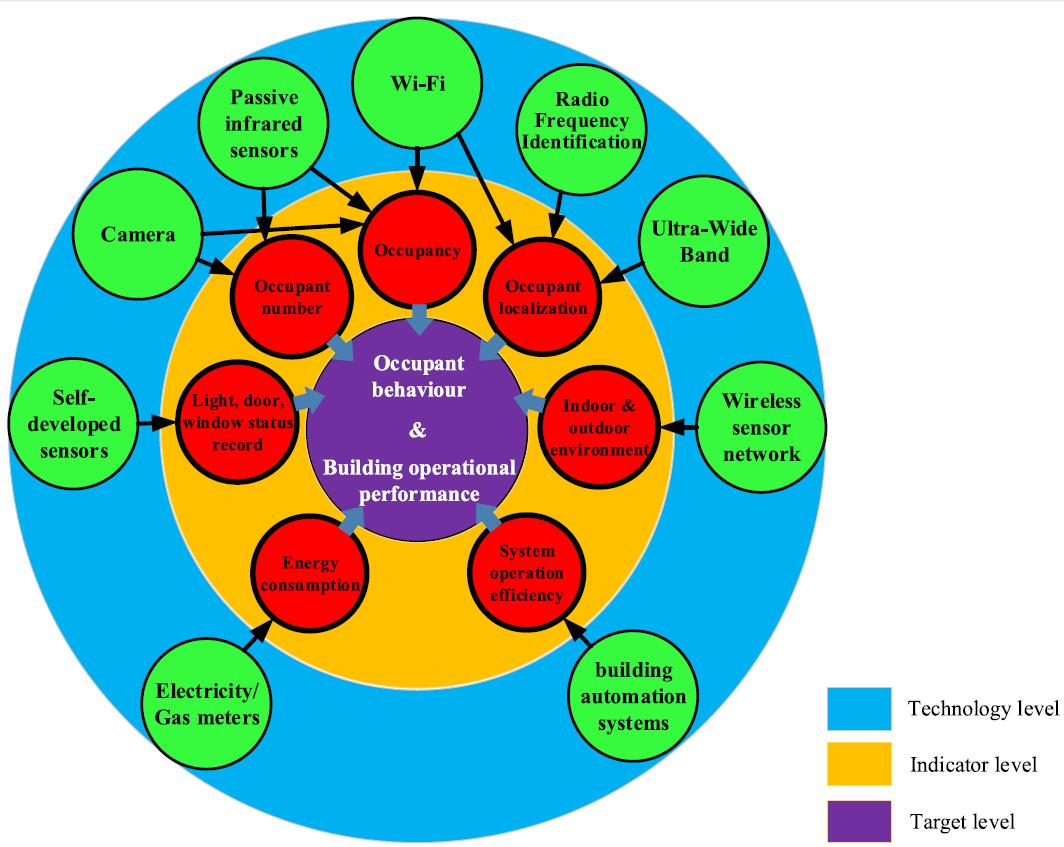
\includegraphics[scale=0.5]{Energy-relatedData.jpg}
			\caption{Technology and method for energy-related data collection \cite{jia2017occupancy}}
			\label{fig:Energy_DataCollection}
			\end{figure}

			\begin{figure}[h!]
			\centering
			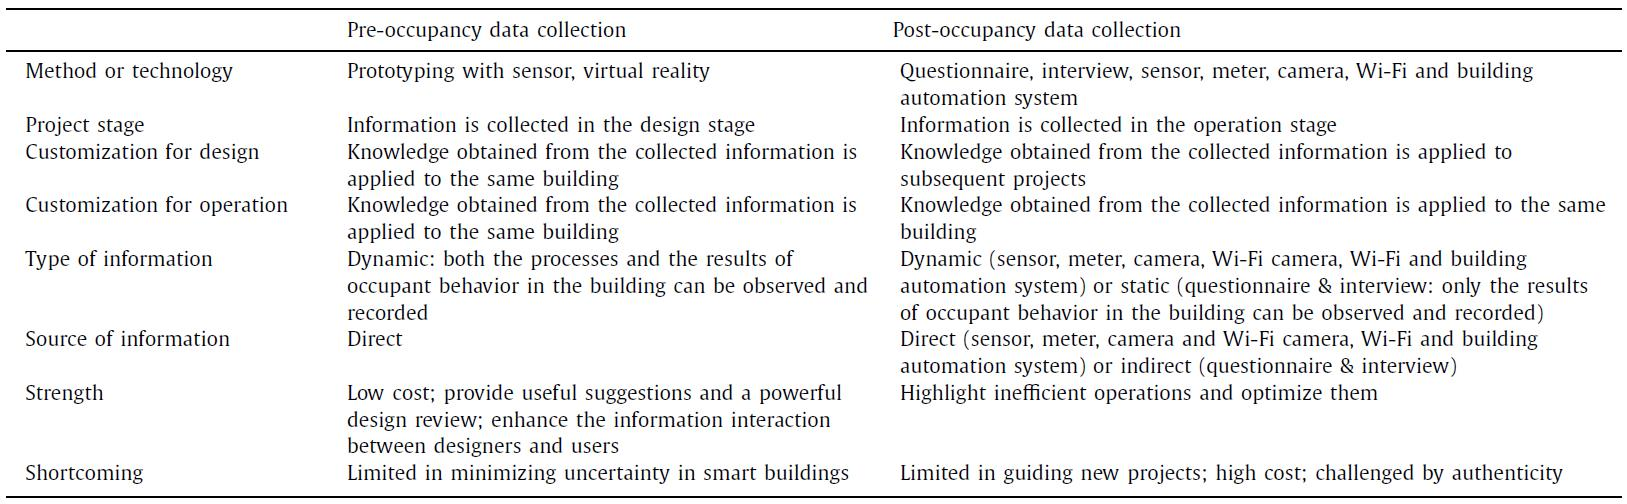
\includegraphics[scale=0.4]{Table1.jpg}
			\caption{Comparison of pre-occupancy data collection and post-occupancy data collection \cite{ZOU2018165}}
			\label{fig:technology1}
			\end{figure}

			\textit{Statistical analysis} is mostly used to develop a numerical relationship among energy consumption, outdoor environment, indoor environment and comfort, occupant behavior and other information using statistical tests, regression analysis and curve fitting \cite{ZOU2018165}. Previous research also show that the above mentioned data collection approaches would be slow and expensive, and the collected data volume is massive and unstructured \cite{liang2016occupancy}.\\

			In order to process this massive amount of data, \textit{Data mining} would be a good technology to structure the collected data and find out the unknown correlations between different data sets. Currently, data mining is used to analyze building energy consumption data and occupancy/occupant behavior data \cite{xiao2014data}.\\

			\textbf{T\&M for occupant behavior modeling and simulation}\\


			\textbf{T\&M for building mechanical system controlling}\\

		\subsubsection{"Soft" Measures}





			


			




	

	\subsection{Selection of Simulation Tools}
		\begin{comment}
		\begin{itemize}
			\item Discuss the existing result of the previous study. 
			\item A significant performance gap is observed. Possible causes of the performance gap.
			\item The data and measurement of previous studies.
			\item Other scientific journals that involve the topic performance gap
		\end{itemize}
		\end{comment}

		
	\subsection{SIA Documentations}
		Introduction of SIA 180 calculation method. Also briefly introduce a set of documentations such as 
		\begin{itemize}
			\item SIA Weather data
			\item SIA dynamic energy analysis
			\item SIA occupancy and schedule
		\end{itemize}
		


		 


\section{Methodology}

	\subsection{SIA Calculation}
		Briefly describe the reason why another SIA calculation is necessary\\
		(Huge gap in building area assumption, huge gap in weather condition)


		\subsubsection{Basic description of SIA Calculation Method}
			Take the floor area and the wall area calculated by DesignBuilder, as there is a significant deviation in \textit{floor area} between the existing SIA calculation and the DesignBuilder model.
			
			\begin{itemize}
				\item Gain
				\begin{itemize}
					\item Solar Gain
					\item Internal Gain (appliance/activities)
				\end{itemize}
				\item Losses
				\begin{itemize}
					\item Transmission Loss (Conduction and Convection)
					\item Ventilation Loss (Air circulation and infiltration)
				\end{itemize}
			\end{itemize}

		\subsubsection{Calculation Assumptions}	
			Two sets of calculation are performed. One uses SIA standard weather condition, the other one uses 2015 weather condition. The 2015 weather data is extracted from the 2015 weather file using Rhino/Grasshopper add-on.
		
		\subsubsection{Measurements expected to close the performance gap}
			Mention a number of suspected parameters which help to help the calculate result reach the historical measurement value.
			\begin{itemize}
				\item Modify the infiltration value
				\item Use correct weather file
				\item Use more accurate floor area
			\end{itemize}


	\subsection{DesignBuilder - Building Modeling}
		A brief introduction of DesignBuilder, also describe the scope of work (Building envelope, create a formated file for EnergyPlus engine, also provide accurate geometry data for SIA calculation)
		
		\subsubsection{Existing Plan}
		Show the building floor plan and functions
		
		\subsubsection{Building Envelope Material}
		A detail description about building envelope material \& U-values \\
		Show the complete building model
		
		\subsubsection{Assumptions}
			\begin{itemize}
				\item Wall/Roof/Ground Floor boundary conditions
				\item Adiabatic boundary conditions
			\end{itemize}
			
	\subsection{EnergyPlus on Nominal Schedule Analysis}
		How did I use EnergyPlus in this Project, and how dose it help me in presenting the data
		
		
		\subsubsection{Schedule and Occupancy Assumptions}
			\begin{itemize}
				\item Detail Schedule and Occupancy Assumptions
				\begin{itemize}
					\item Occupancy
					\item Schedule
					\item Activity level
					\item Lighting / new-lighting schedule
					\item DHW
					\item Electricity
				\end{itemize}
				
				\item Shading
				\item Documentation base (SIA xxx)

			\end{itemize}
			
		\subsubsection{Weather Data Selection}
			\begin{itemize}
				\item Data source: IDAweb
				\item Weather data selection base: location,date
				\item Weather file modification (replaced parameters)
					\begin{itemize}
						\item Temperature (dry/wet)
						\item Relative Humidity
						\item Wind speed
						\item Wind direction
					\end{itemize}
			\end{itemize}
			

	

	\subsection{jEPlus Dynamic Simulation}
		Why using je-Plus and how to use
		\subsubsection{Basic description of je-Plus}
		\begin{itemize}
			\item Main functions
			\item Advantages
			\item How to use
		\end{itemize}
	
		\subsubsection{Dynamic Parameter Assumptions}
		List of parameters, range of parameters and distribution of parameters


	\subsection{Calibration}
		In order to ensure the simulated buildings have similar thermal behaviors as the real buildings, a calibration to the building envelope is needed.
		The calibration process needs to be in a summer period where no heating and cooling is performed. The calibration should vary the building tightness and basic appliance schedules until the calculated indoor environment (temperature in this case) behaves similar enough to the historical measurement.
		

		\subsubsection{Outdoor Environment Calibration}
		\subsubsection{Building Envelope Calibration}
		\begin{itemize}
			\item EnergyPlus Hourly Analysis
		\end{itemize}


	
	\subsection{Data Processing}
		Briefly describe the resulting data structure from je-Plus and introduce 2 different graphs.
		\subsubsection{Dynamic Analysis Range}

		\subsubsection{Correlation Matrix}
		An introduction about Correlation matrix

\section{Results}

	\subsection{Initial Annual Energy Analysis}
		\subsubsection{SIA Calculation}
			Compare the results
			\begin{itemize}
			 	\item Previous Result (by Lemon Consult)
			 	\item Apply correct building floor and wall area
			 	\item Apply year 2015 weather data
			 	\item Modify air tightness (infiltration)
			 	\item Historical measurement value
			 \end{itemize}
			  
		\subsubsection{EnergyPlus Simulation Result}		
		\begin{itemize}
			\item Floor Area (be used in SIA calculation)
			\item Heating Demand
			\item Air Ventilation
		\end{itemize}
		The first set of dynamic analysis (4 sets of heating demand distribution from infiltration 0.1 to 0.4)


		\subsubsection{Calibration}
			\begin{itemize}
				\item Steps of calibration (hourly - annually)
				\item Results of each variation (new lighting schedule/shading schedule etc)
				\item Recommended base values
			\end{itemize}
			
		\subsubsection{jE-Plus Simulation Results}
			\begin{itemize}
				\item Dynamic Heating Demand Variation
				\item Dynamic DHW Demand Variation
				\item Results of all parameters (range and distribution of heating demand and DHW demand)
				\item Correlation of parameters
			\end{itemize}



\section{Discussion}

		\begin{itemize}
		\item Key parameters (Which parameters are the most important and which are not as important)
		\item Key assumptions (Are these assumption still applicable)
		\item Recommendation (building envelope much be accurate, a weather data update is critical etc)
	\end{itemize}
			
\section{Conclusion}
	\begin{itemize}
		\item Key parameters
		\item Recommended set of parameters
		\item General Recommendations
	\end{itemize}


%\section{Reference}

\printbibliography







\end{document}




%%%
%%	\end{multicols*}
%	\end{landscape}
